% Drawing 64/02-1 -- folder 64, batch 02, archive page 35 (PDF page 36).
% Transcription: tableau (40), première colonne : un cube en perspective dont les huit sommets sont marqués alternativement d'un point plein et d'un petit cercle (les sommets des deux tétraèdres inscrits).
% Kind: cube with vertices marked alternately full and open. Method 2 (schematic redraw from the facsimile). Status: ok.
% Notes: The cube in perspective, twelve edges drawn between the eight vertices, each vertex full or open as on the page: front face (lower left of the picture) upper left full, upper right open, lower right full, lower left open; back face upper left open, upper right full, lower right open, lower left full; so every edge joins a full vertex to an open one. The edges of the back face that are hidden (the lower one and the left one) are drawn dashed, as he broke them. The ring of the back lower right vertex is partly filled with ink on the page: read open, as the alternation requires. Redrawn 2026-11-12 (issue 128): to check again.
% Coordinates: 1 unit = 0.45 mm = 1/100 of the crop width (bbox in page fractions: [0.27, 0.14, 0.38, 0.21]).
% Redrawn by Claude (claude-fable-5-2), issue #128, 2026-11-12; not checked by a human; not compiled (no TeX in the session).
% Rights: reproduces part of the work -- behind RENDER_TRANSCRIPTS, never published by itself.
\documentclass[tikz,border=3pt]{standalone}
\usepackage{amsmath,amssymb}
\usetikzlibrary{patterns,arrows.meta}
\tikzset{pencil/.style={black!45}, struck/.style={black!35}, mpt/.style={circle,draw,inner sep=1.3pt}, pt/.style={circle,fill,inner sep=0.9pt}, opt/.style={circle,draw,fill=white,inner sep=1.1pt}}
\begin{document}
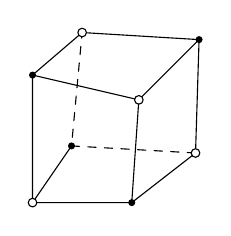
\begin{tikzpicture}[x=0.45mm,y=0.45mm,line cap=round,line join=round,font=\scriptsize]
\draw (19,-40) -- (49,-47) -- (47,-76) -- (19,-76) -- cycle;
\draw (33,-28) -- (66,-30) -- (65,-62);
\draw[dashed] (65,-62) -- (30,-60) -- (33,-28);
\draw (19,-40) -- (33,-28);
\draw (49,-47) -- (66,-30);
\draw (47,-76) -- (65,-62);
\draw (19,-76) -- (30,-60);
\node[pt] at (19,-40) {};
\node[pt] at (47,-76) {};
\node[pt] at (66,-30) {};
\node[pt] at (30,-60) {};
\node[opt] at (49,-47) {};
\node[opt] at (19,-76) {};
\node[opt] at (33,-28) {};
\node[opt] at (65,-62) {};
\end{tikzpicture}
\end{document}
